\section{Experiment}

\begin{frame}{实验}
    \begin{scriptsize}
        \begin{figure}
            \centering
            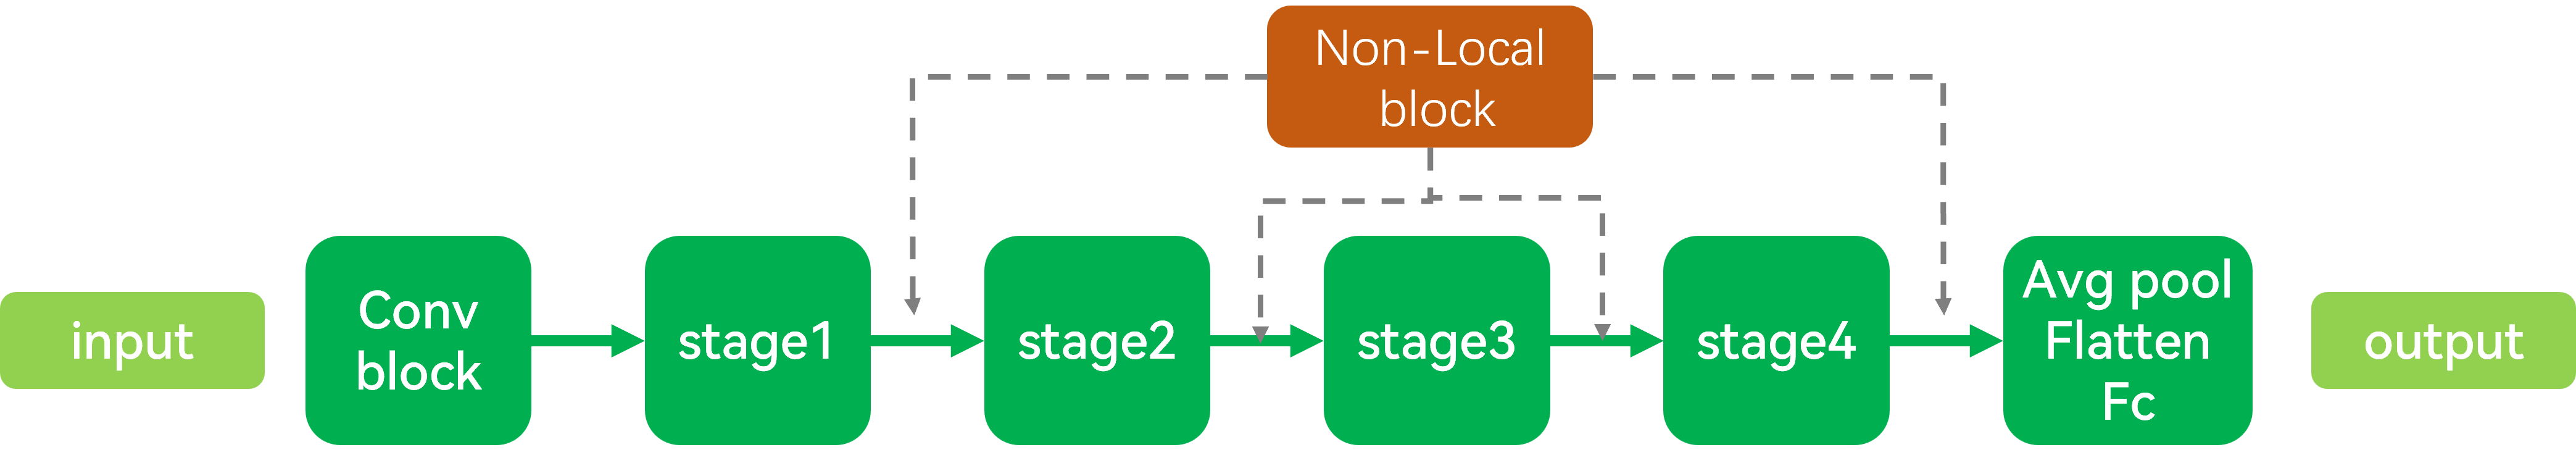
\includegraphics[width=0.9\textwidth]{docs/0903/images/resnet-nonlocal.png}
        \end{figure}
        Baseline选择ResNet-50,不同stage加入non-local模块,进行对抗训练
        \begin{table}
            \begin{tabular}{ccc}
                \hline
                模型 & 干净样本训练 & 对抗训练(FGSM生成对抗样本) \\  
                \hline          
                ResNet-50                       & 0.9380 & 0.9325 \\
                ResNet-50(Non-Local in layer-1) & 0.9365 & 0.9275 \\
                ResNet-50(Non-Local in layer-2) & 0.9420 & 0.9285 \\
                ResNet-50(Non-Local in layer-3) & 0.9455 & 0.9145 \\
                ResNet-50(Non-Local in layer-4) & 0.9310 & 0.9035 \\
                \hline          
            \end{tabular}
        \end{table}
        
        问题:模型训练的时候,在不同epoch的结果不一样,那么一些论文中的结果是怎么确定的呢?并且数据的差异很小,0.**的差异
    \end{scriptsize}    
\end{frame}

\begin{frame}{实验}
    % \begin{figure}
    %     \centering
    %     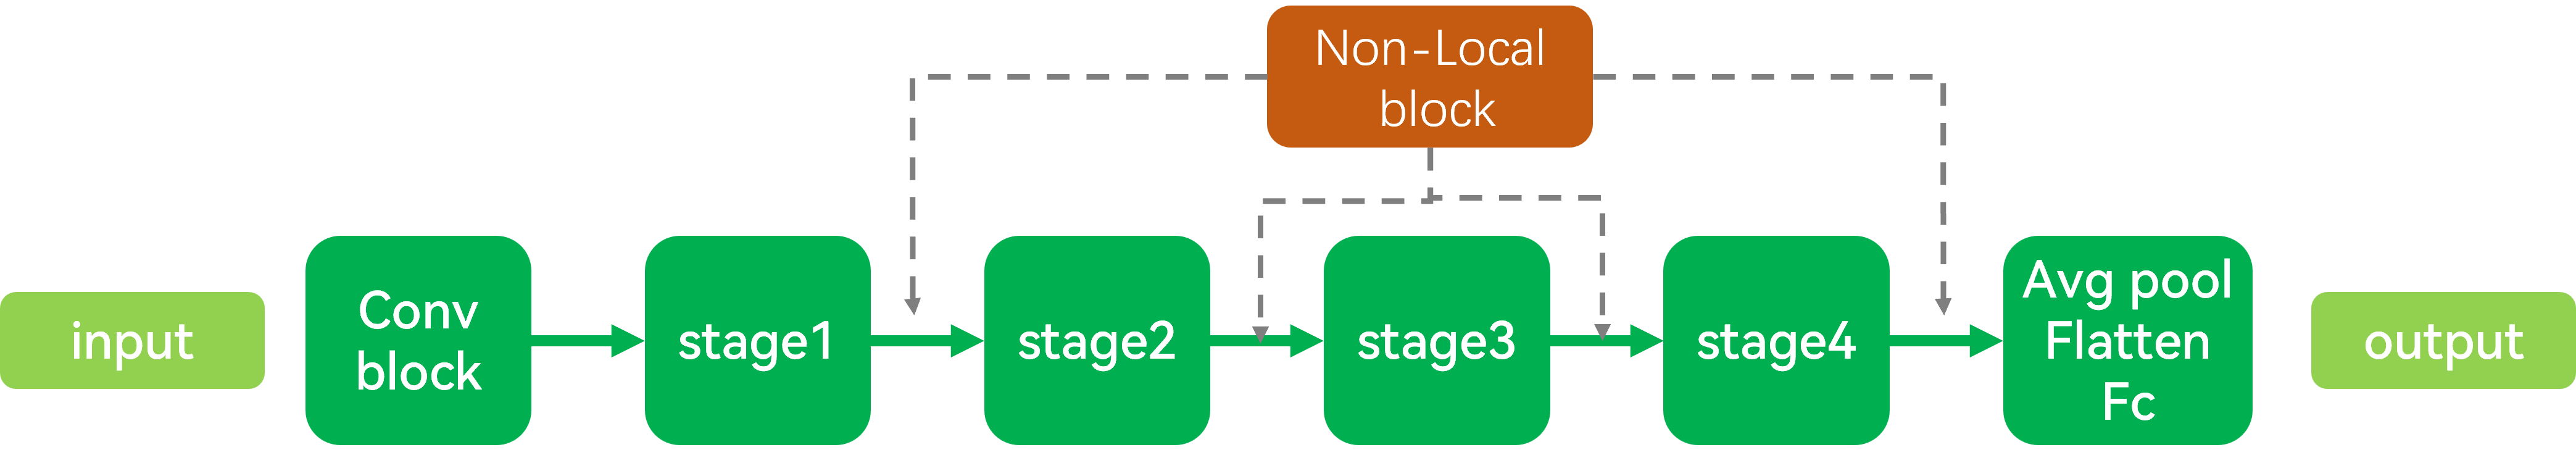
\includegraphics[width=0.7\textwidth]{docs/0903/images/resnet-nonlocal.png}
    % \end{figure}

    在模型微调的时候,如果想在模型中加入不同的模块验证他们的作用(消融实验?),在自己训练完成之后的模型(ResNet50)有BN层参数,但是加载模型库里面的模型没有BN层,那这个时候会不会对结果有影响之类的(好像没有办法把这些训练好的BN层的参数加载到新的模型上)
    \begin{figure}
        \centering
        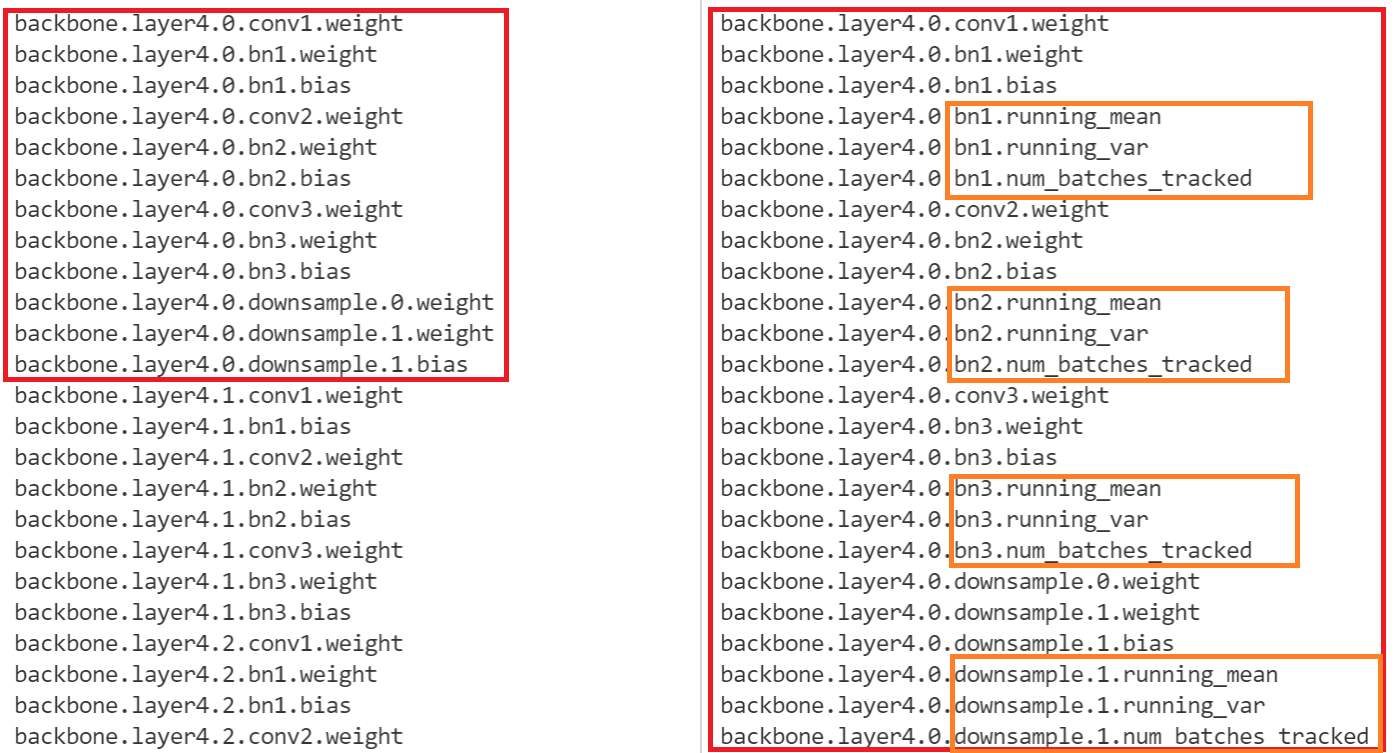
\includegraphics[width=0.6\textwidth]{docs/0903/images/s.png}
    \end{figure}
\end{frame}